99. По теореме Виета $x_1+x_2=a^2-5a=a(a-5)<0\Rightarrow a\in(0;5).$ Также необходимо проверить существование корней, то есть $D=(a^2-5a)^2-16=
(a^2-5a-4)(a^2-5a+4)=$\\$\left(a-\cfrac{5-\sqrt{41}}{2}
ight)\left(a-\cfrac{5+\sqrt{41}}{2}
ight)(a-4)(a-1)\geqslant0.$\\ Применив метод интервалов, найдём ответ:
\begin{figure}[ht!]
\center{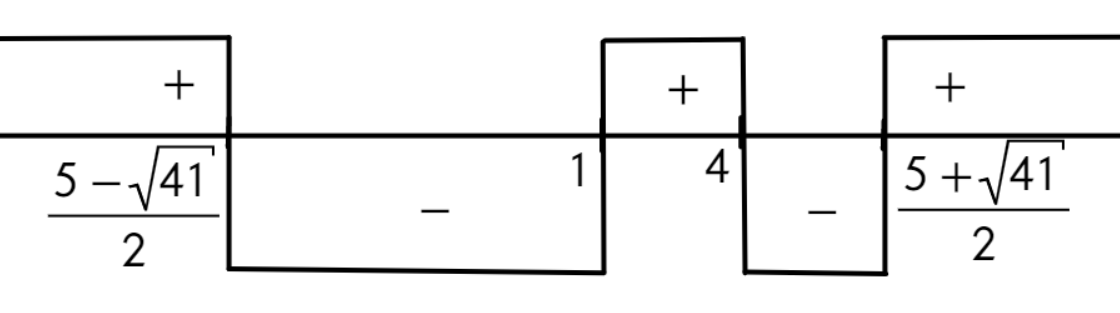
\includegraphics[scale=0.35]{isl99.png}}
\end{figure}
$a\in\left(-\infty;\cfrac{5-\sqrt{41}}{2}
ight]\cup[1;4]\cup\left[\cfrac{5+\sqrt{41}}{2};+\infty
ight).$
Окончательным ответом в задаче будет пересечение полученных ответов, $a\in [1;4].$\\
